\subsection{JavaScript}
JavaScript\index{JavaScript} ist eine Programmiersprache, die beim Ausführen, also z. B. beim Aufruf einer Webseite, von einem entsprechenden Programm interpretiert wird, und sie zählt somit zu den Interpreter-Sprachen. Zudem ist es eine schwach typisierte Sprache, das heißt, einer Variablen wird nicht explizit ein Typ zugewiesen, sondern sie erhält diesen implizit durch seinen Wert.
JavaScript wurde für den Einsatz innerhalb von Webseiten entworfen, wird heutzutage aber auch auf Servern verwendet. So werden Module für Node.js (\autoref{sec:nodejs}) in JavaScript geschrieben.\\
Bei JavaScript handelt sich um eine Implementation von ECMAScript\index{ECMAScript}, welche von Ecma International unter der Bezeichnung ECMA-262  spezifiziert wird, und sie wurde im Juni 2016 in der mittlerweile siebten Version veröffentlicht \cite{International2016}. Neuere Versionen bieten Sprachkonstrukte wie Module, Klassen und vieles mehr an. Jedoch unterstützen die Browser oder besser gesagt deren Interpreter bis dato nicht alle neuen Funktionen, wie \autoref{tab:ecmasupport} zu entnehmen ist. \\
\begin{minipage}{\textwidth}
\begin{longtable}{|c||c|c|c|}
	\hline  
	\backslashbox{\thead{Browser}}{\thead{Version}}& \thead{ECMAScript 5} & \thead{ECMAScript 6} & \thead{ECMAScript 7} \\  \hhline{|=||=|=|=|}
	\thead{Chrome 51} & 98 \% (Seit CH23+) & 98 \%  & 25 \% \\ 
	\hline 
	\thead{Firefox 47} & 100 \% (Seit FF21+) & 90 \% & 29 \% \\ 
	\hline 
	\thead{Safari 9} & 96 \% (Seit SF6+) & 53 \% & 1 \% \\ 
	\hline 
	\thead{Edge 13} & 99 \% (Seit IE10+) & 79 \% & 7 \% \\ 
	\hline 
	\thead{Android Browser 5.1} & 98 \% (Seit AN 4.4+)  & 29 \% & 4 \% \\ 
	\hline 
	\thead{iOS Safari 9} & 96 \% (Seit SF6+) & 53 \% & 1 \%\\ 
	\hline
	\caption{Ausschnitt der Browserunterstützung von ECMAScript \cite{ecmasupport}}\label{tab:ecmasupport}
\end{longtable}
\end{minipage}

Zu erkennen ist, dass gängige Browser in ihrer aktuellen Version weder Version 6 noch Version 7 zuverlässig unterstützen, wohingegen ECMAScript 5 in den meisten Browsern seit geraumer Zeit großteils lauffähig ist. Soll auch älteren Browsern der Zugriff auf eine Webpräsenz gewährleistet werden, so sollte man auf den Standard ECMAScript 3 aus dem Jahr 1999 zurückgreifen, da alle in \autoref{tab:ecmasupport} diese zu mindestens 96 \% unterstützen.\\
Zu beachten ist, dass in dieser Arbeit JavaScript als Synonym für ECMAScript steht. JavaScript ist lediglich eine Implementierung von ECMAScript der Organisation Mozilla Foundation. Jedoch werden aus geschichtlichen Gründen heute beide Begriffe oft als Synonym gehandhabt.

Mit JavaScript ist es möglich, auf Eingaben und Interaktionen des Anwenders zu reagieren und das Erscheinungsbild der Webseite dynamisch, ohne dass diese komplett neu geladen werden muss, zu verändern. Dies erfolgt durch Manipulation des \ac{dom}\index{DOM}, wobei es sich um eine Schnittstelle für den Zugriff auf ein HTML-Dokument handelt. Über die Schnittstelle lassen sich Knoten in einer Baumstruktur ablegen. Die durch das \autoref{lst:html} generierte HTML-Seite würde wie folgt aussehen.
\begin{figure}[H]
    \begin{center}
        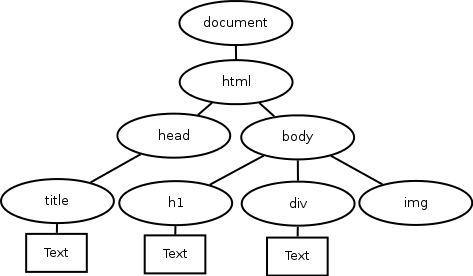
\includegraphics[width=.8\textwidth]{dom.png}
        \caption{Vereinfachte Baumstruktur des DOM ohne Attribute}
        \label{img:dom}
    \end{center}
\end{figure}

Der JavaScript-Code befindet sich innerhalb des HTML-Dokumentes in einem Script-Element, oder er wird als externe JavaScript-Datei in das HTML-Dokument eingebettet. Im folgenden Codebeispiel soll gezeigt werden, wie man ein Dokument mittels DOM-Manipulation beeinflussen kann.

\begin{lstlisting}[style=htmlcssjs, caption=Ein JavaScript Beispiel, label=lst:javascript]
<script>
  document.getElementById("inhalt").innerHTML="Ein neuer, Text!";
</script>
\end{lstlisting}

Es wird im Dokument aus \autoref{img:html} das Element mit dem id-Attribut und dem Wert \quotes{inhalt} gesucht und dessen Inhalt ersetzt. Der Text \quotes{Meine erste Webseite!} lautet nun: \quotes{Ein neuer Text!}. Zur DOM-Manipulation gehört auch die Möglichkeit, Elemente zu löschen, neue einzufügen und deren Attribute zu bearbeiten.\\